\chapter{Introduction and overview}

Several species of fish share an uncommon sense, making them able
to probe their surrounding environment thanks to a self-generated
electric field. Very much like bats, which use a sonar to orient themselves,
these fishes are equipped with some sort of radar. Indeed, they are
able to create an electric potential thanks to a special organ, which
is then recorded by specific sensors located at the surface of their
skin. This allows them to perceive the distorsion created
by the presence of a target, which gives them access to the size,
the shape, and the material of this object. This ability is called
\emph{active electrolocation} and was discovered by Hans Lissmann
and Ken Machin in 1958~\cite{lissmann1958mechanism}.

Since this finding, a huge amount of work has been done in order to
understand this sense. However, a quantitative model is lacking to
explain the physics that underly within this low-frequency imaging
technique. In this perspective, it is interesting to investigate what
are the equations involved, the relevant parameters, and the phenomena
that could furnish a satisfying explanation.

From a mathematical point of view, this problem is promising since
it gives an example of an \emph{inverse problem} solved by the fish.
Hence, the study of its behaviors could lead us to invent numerical
algorithms that could avoid the ill-posedness of such problems. Biomimetism
and bio-inspired technologies are then not very far from this approach.

\medskip{}


In this chapter, we will first focus on the electric fishes (section~\ref{sec:state-of-the-art}),
and then we will present the main outline of the work presented in
this thesis (section~\ref{sec:overview}).


\section{State of the Art}

\label{sec:state-of-the-art}

This section presents, in a non-exhaustive way, what is known about
electric fishes. The interested reader should refer to \cite{neuro,moller1995electric},
two remarkable reviews on the subject from which the following lines
have taken their sources.


\subsection{Discovery of the Electric Sense: a Brief History}

The relations between man and electric fishes teach us how the study
of these latters improved scientific knowledge, from the invention
of the first electric battery to the finding of acetylcholin. This
section intends to summarize this long scientific journey, showing
that -~starting with electrolocation~- mysteries to be uncovered
still hold. It relies heavily on~\cite{finger2011shocking,moller1995electric};
the first reference is a must-read which is accessible for any public.

\paragraph{Bioelectrogenesis}
One of the most ancient trace of knowledge of these fishes can be
found on the Narmer Palette, depicting King Narmer (Early Dynastic
Period, 31st century BC) whose name is composed by the two symbols
\emph{n'r} (catfish) and \emph{mr} (chisel), see Figure~\ref{fig:Narmer-Palette}.

\begin{figure}
\centering%
\begin{tabular}{cc}
\includegraphics[height=6cm]{intro/figures/narmerp1} & 
\includegraphics[height=3cm]{intro/figures/serekh}\tabularnewline
\end{tabular}
\caption{\label{fig:Narmer-Palette}The Narmer Palette (left), and a zoom on
the \emph{serekh} (box containing the name) situated on the top (right)
The fish that is represented is probably \emph{Malapterurus electricus}~\cite{boulenger1965fishes,howes1985phylogenetic}.}
\end{figure}

The electric shocks were then also used in medicine, as being analgesic; this practice
seems to have endured during Ancient Greece.

The link between those shocks and thunders had been a mystery since, until the
$18$th century, helped by the Leyden jar. Officialy, John Walsh
is rewarded for this discovery (receiving the Copley Medal of The Royal Society
in $1775$). However, a lot of people had recognized the electrical nature of
the discharges of the electric eel, the torpedo or the electric catfish:
Hunter ($1773$), van s'Gravesande ($1754$), van der Lott ($1762$), Bancroft ($1769$),
Bajon ($1774$), Williamson ($1775$) and Cavendish ($1776$). A surprizing fact
tells us that the first electric battery (built by Volta in $1800$) was designed
to be an electric organ; more details will be given on that point in 
subsection~\ref{subsub:emit-receive-field}.

At the end of the $19$th century, weakly electric fishes are discovered. In the
perspective of the freshly established theory of evolution by Darwin, the question
of the use of such a low signal is raised. Indeed, a few millivolts is no use
for harming a prey.

At the beginning of the $20$th, Fledberg and Fessard study the electric organ
of the Torpedo in order to demonstrate that acetylcholine is a
neurotransmitter~\cite{feldberg1942cholinergic}.

\paragraph{Electroreception}
John Walsh and his contemporaries -~Ingenhousz ($1782$), Schilling ($1772$) and
Faraday ($1839$)~- remarked that these fishes ``feel'' electricity. Electroreceptor
organs were discovered by Lorenzini in $1678$ but the link between emission and
reception is not made; Du Bois-Reymond and Müller went to reject it. It is only
in $1958$ that Lissmann and Mahcin showed that these organs were part of a
complex electroperception system, allowing these fishes not only to probe their
environnement, but also to communicate between them. 


\subsection{Weakly Electric Fish}


\subsubsection{Taxonomy and living conditions}

There are dozens of weakly electric species, classified in various
families. These families all belong to two different orders: Gymnotiforms
in South America and Mormyriforms in Africa (see Figure~\ref{fig:geography}).

\begin{figure}[!h]
\centering
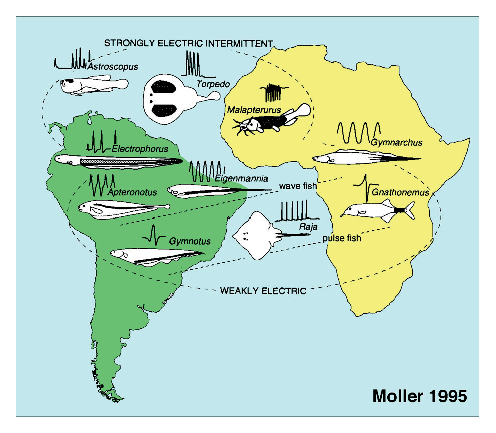
\includegraphics[width=12cm]{intro/figures/fish_geography.eps}
\caption{Classification and geographic distribution of the different species of weakly electric fish. The species of interest are in the lower circle and the other ones use their electric organ in an aggressive or defensive manner. Taken from~\cite{moller1995electric}. \label{fig:geography}}
\end{figure}

These fishes hunt at night and sleep during the day. They live in muddy rivers,
therefore the turbidity of the water is very high. However, as we will see in
chapter~\ref{chap:math-model}, only conductivity will have an importance on electrolocation.
This latter is considered to be homogenized because of the little size of the particles
suspended in the water.

The shape and size of these fishes vary considerably from one species to
another. Two types are distinguished according to the electric signal
emitted: pulse-type species and wave-type species (see Figure~\ref{fig:pulse_wave}).

\begin{figure}[!h]
\centering

\includegraphics[width=10cm]{intro/figures/pulse_wave}
\caption{Differences between two species: one is pulse-type (top) and the other is wave-type. For each fish, its electric discharge is represented in time scale. Taken from \cite{graff2004fish}. \label{fig:pulse_wave}}
\end{figure}


\subsubsection{Emitting and receiving the electric field}
\label{subsub:emit-receive-field}

This section will explain the physical, chemical and biological mechanisms
involved during \emph{electrogenesis} and \emph{electroreception}.

Whatever the type of specie (wave or pulse), the emission relies on
the same principle and is due to a specific organ which is generally
situated in the tail;~the first paragraph will provide more details.
The reception is operated by receptors spreading on the surface of
the skin; further explanation will be given later on.


\paragraph{The electric organ}

Apart from the family Apteronotidae (in the Gymnotiforms order), the
Electric Organ (denoted \emph{EO} below) emitting the electric discharges
derives from muscular tissues - it is called \emph{myogenic organ}
- built in superimposed disks (cf Figure \ref{fig:electric_organ}).
These disks are in fact big cells ($0.75$~mm in \emph{Brachyhypopomus
pinnicaudatus}~\cite{stoddard2008signal}) called \emph{electrocytes}.
Their number ranges from hundreds (in Mormyrids) to several millions
in strongly electric species.

\begin{figure}[!h]
\centering
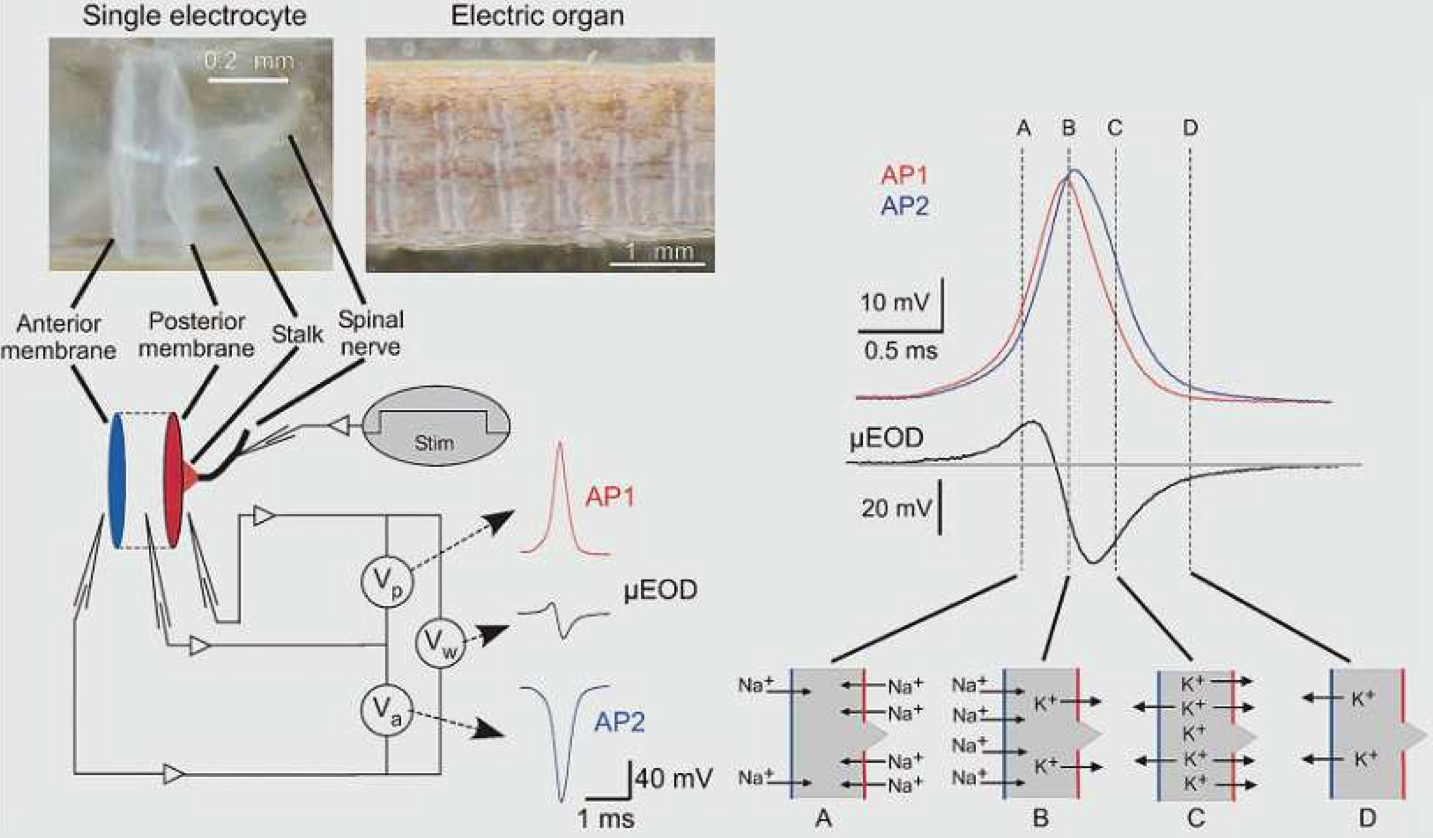
\includegraphics[width=\textwidth]{intro/figures/electric_organ}
\caption{A \emph{Brachyhypopomus pinnicaudatus} electrocyte. Taken from \cite{stoddard2008signal}. \label{fig:electric_organ}}
\end{figure}

An \emph{Electric Organ Discharge} (denoted \emph{EOD} below) is as
follows: first, the brain sends an impulse that goes through a pacemaker
in the spinal cord. This pacemaker is connected to every electrocyte
by a \emph{spinal nerve}. Each nerve depolarizes the caudal (\emph{i.e.}
posterior) part of the cell, which causes the opening of the ionic
canals situated on the membrane (they are uniquely sensible to voltage
difference between the interior and the exterior of the cell). It
follows a ionic flux (see A, B, C and D in Figure\inputencoding{latin1}{~}\inputencoding{latin9}\ref{fig:electric_organ})
that makes the electric current. It should be noted that the great
similarity with a battery is historic: indeed, Volta built its first
pile in 1800 according to his observations of the eel's organ~\cite{volta1800electricity}
and named it \emph{Artificial Electric Organ}.

However, in Apteronotidae species the EO derives from neural tissues
and therefore is said to be \emph{neurogenic}. In this case, the organ
is composed of several presynaptic axons of electromotor nerves (see
Figure~\ref{fig:neurone}) that are not connected at their end. When
the brain sends a signal in these neurons, the sum of all the small
currents makes the discharge.

\begin{figure}
\centering
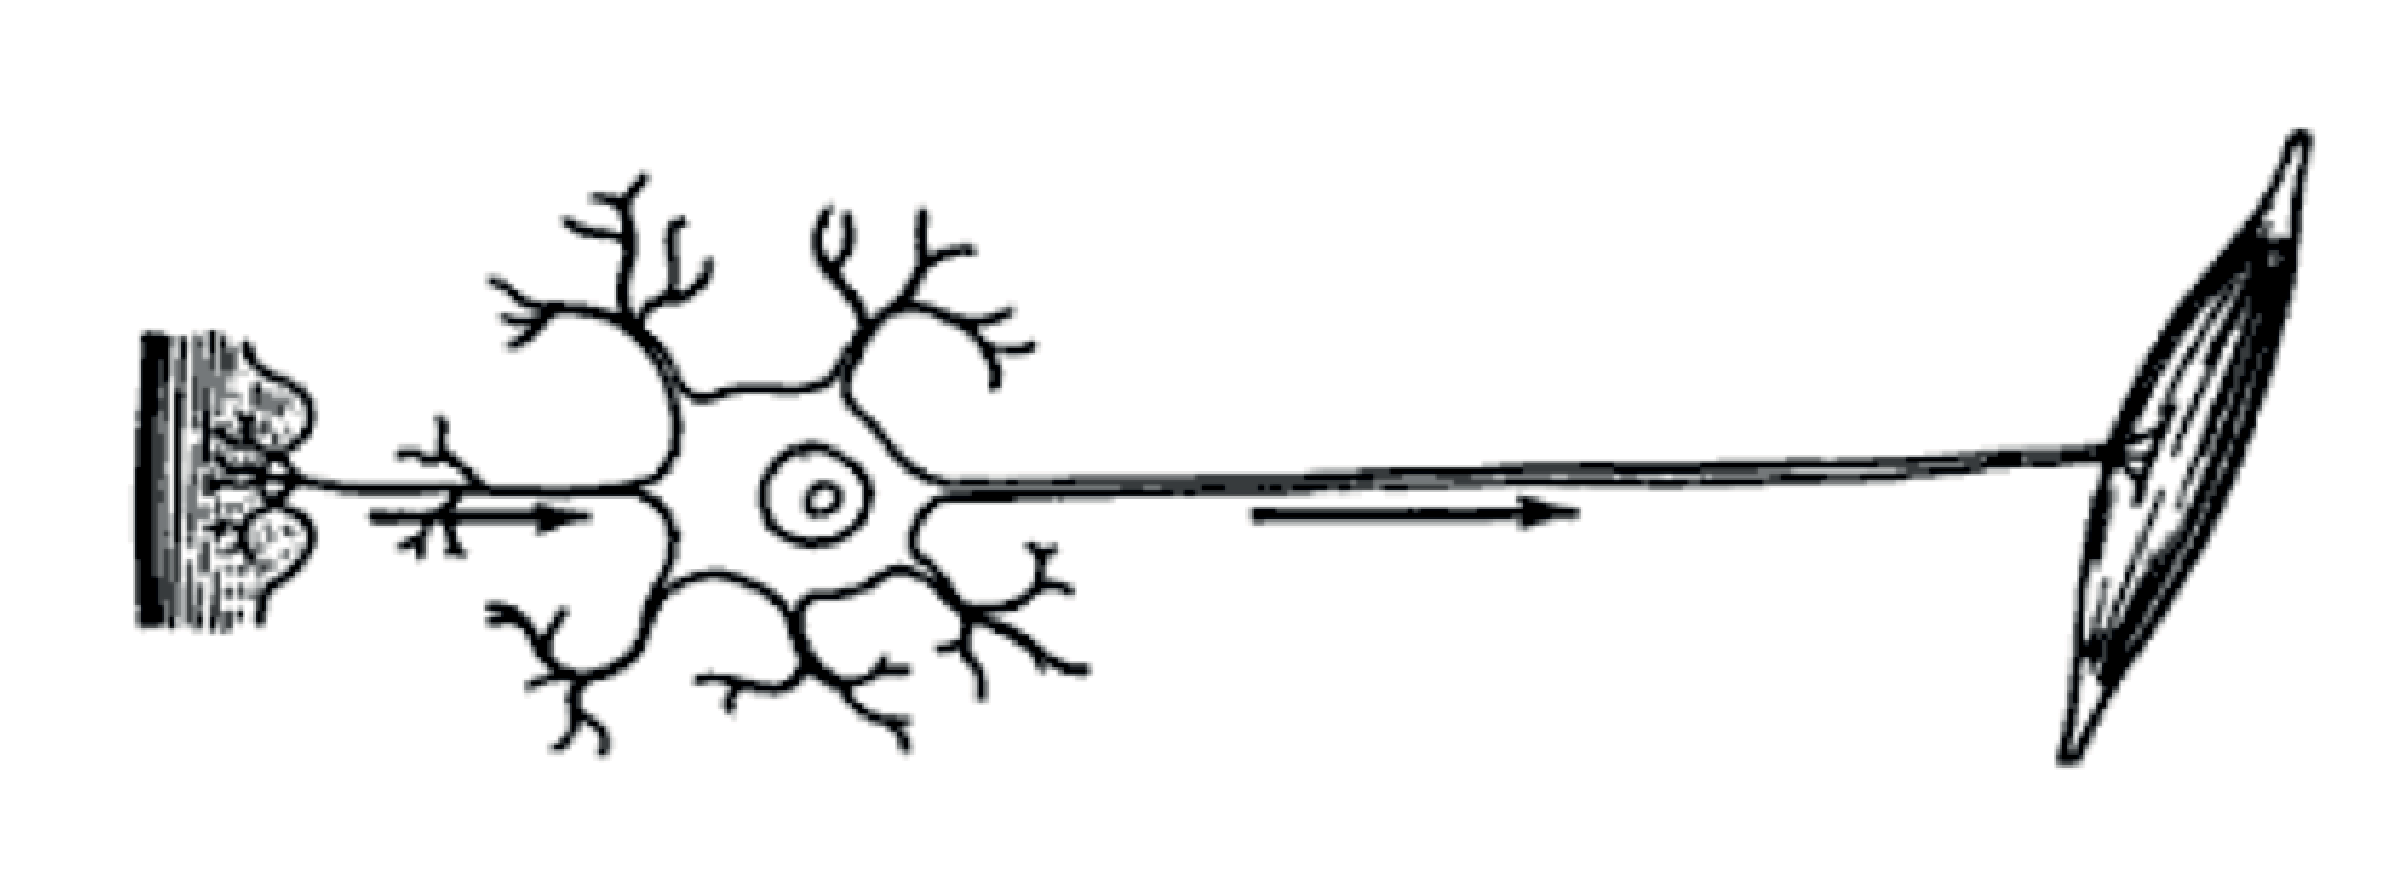
\includegraphics[width=7cm]{intro/figures/neurone}
\caption{An electromotor neuron. The axon connects the body of the neuron (in the center) to the muscular tissues (on the right). Taken from \cite{rouviere2002}. \label{fig:neurone}}
\end{figure}

Depending on the species, this organ occupies a small part of the
body (for example in Mormyrids it is located in the caudal peduncle)
or an extended one (for example almost the entire trunk in Gymnarchus
niloticus).


\paragraph{Electroreceptors}

\label{sub:electrorecepteurs}

There are thousands of pores - sizing around a millimeter - on its
scaleless skin. In each of them can be found an electroreceptor used
to measure the voltage difference between the exterior medium and
the inside of the fish's body. A receptor is formed by a cavity filled
by a conducting material (liquid or fibers): when a potential difference
is applied a current appears in this material, which is measured by
sensitive cells (see Figure\inputencoding{latin1}{~}\inputencoding{latin9}\ref{fig:electroreceptor}).
Then this information is transmitted to the brain via \emph{afferent
neurons}.

Two types of receptors are distinguished according to their shape:
\emph{ampullary} receptors and \emph{tuberous} ones. The shape is
not the only difference, since the ampullary receptors measure low
frequency signals (from $1$ to $10$~Hz) and the others are sensitive
to high frequencies (from a hundred of Hertz to $1$~kHz). Moreover,
the laters can be either sensitive to the amplitude of the signal
(in this case they are called AM for \emph{Amplitude-Modulating units})
or to the frequency (here they are called RT for \emph{Rapid Timing
units}).

\begin{figure}[h]
\centering
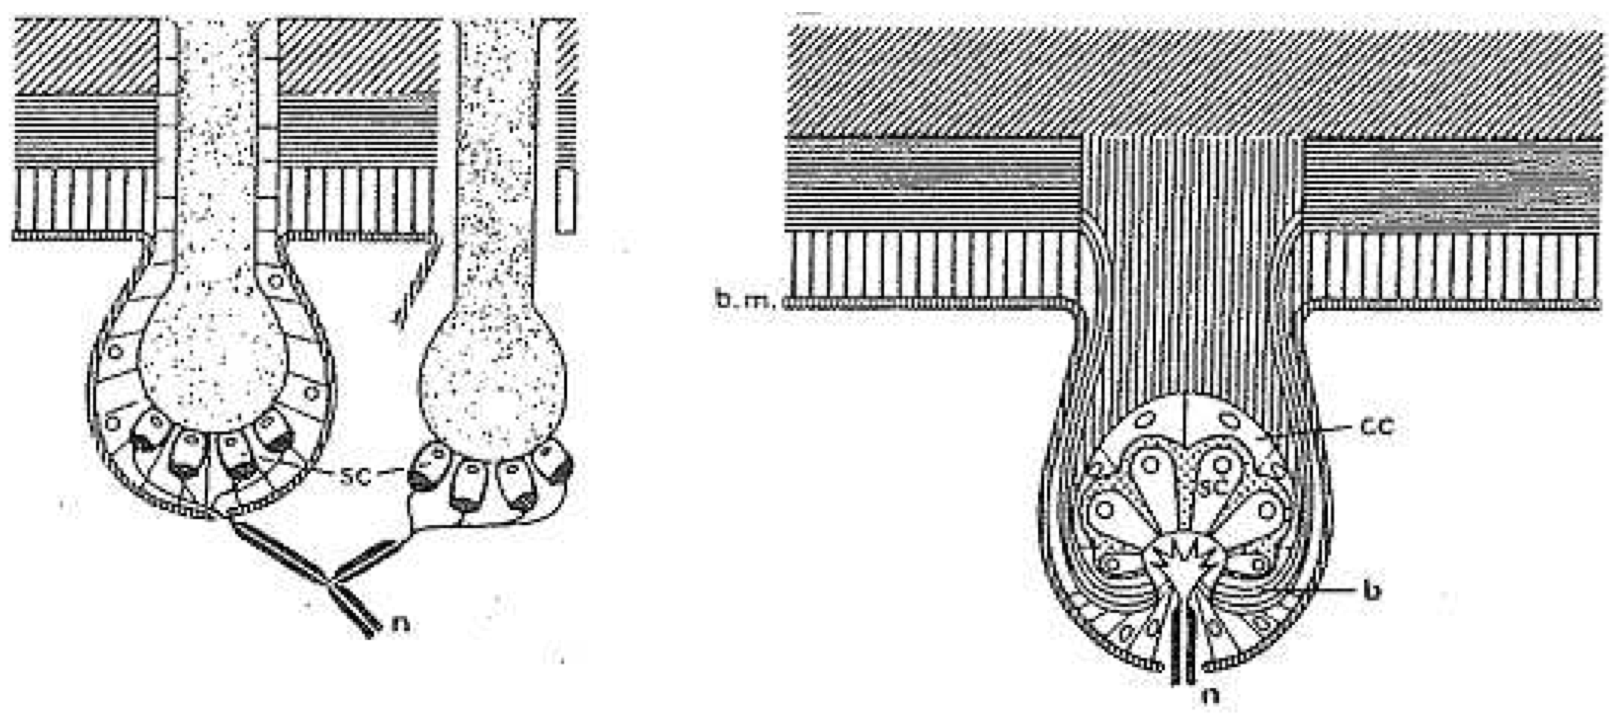
\includegraphics[width=13cm]{intro/figures/electroreceptors}
\caption{Two types of electroreceptors: an ampullary receptor on the left (this shape is common to Mormyrids and Gymnotiforms) and a tuberous one on the right (this shape of organ is from Gymnotiforms). Sensitive cells are indicated by {}``sc'' and the afferent neurons are noted {}``n''. Taken from \cite{moller1995electric}. \label{fig:electroreceptor}}
\end{figure}

However the repartition on the skin depends on the species, there
are similarities in each order. Indeed, it is rather uniform in Gymnotiforms
(though the density is higher near the head) and it is concentrated
on the back and on the ventral part of the body in Mormyriforms (see
Figure~\ref{fig:density_electroreceptor}).

\begin{figure}[h]
\centering
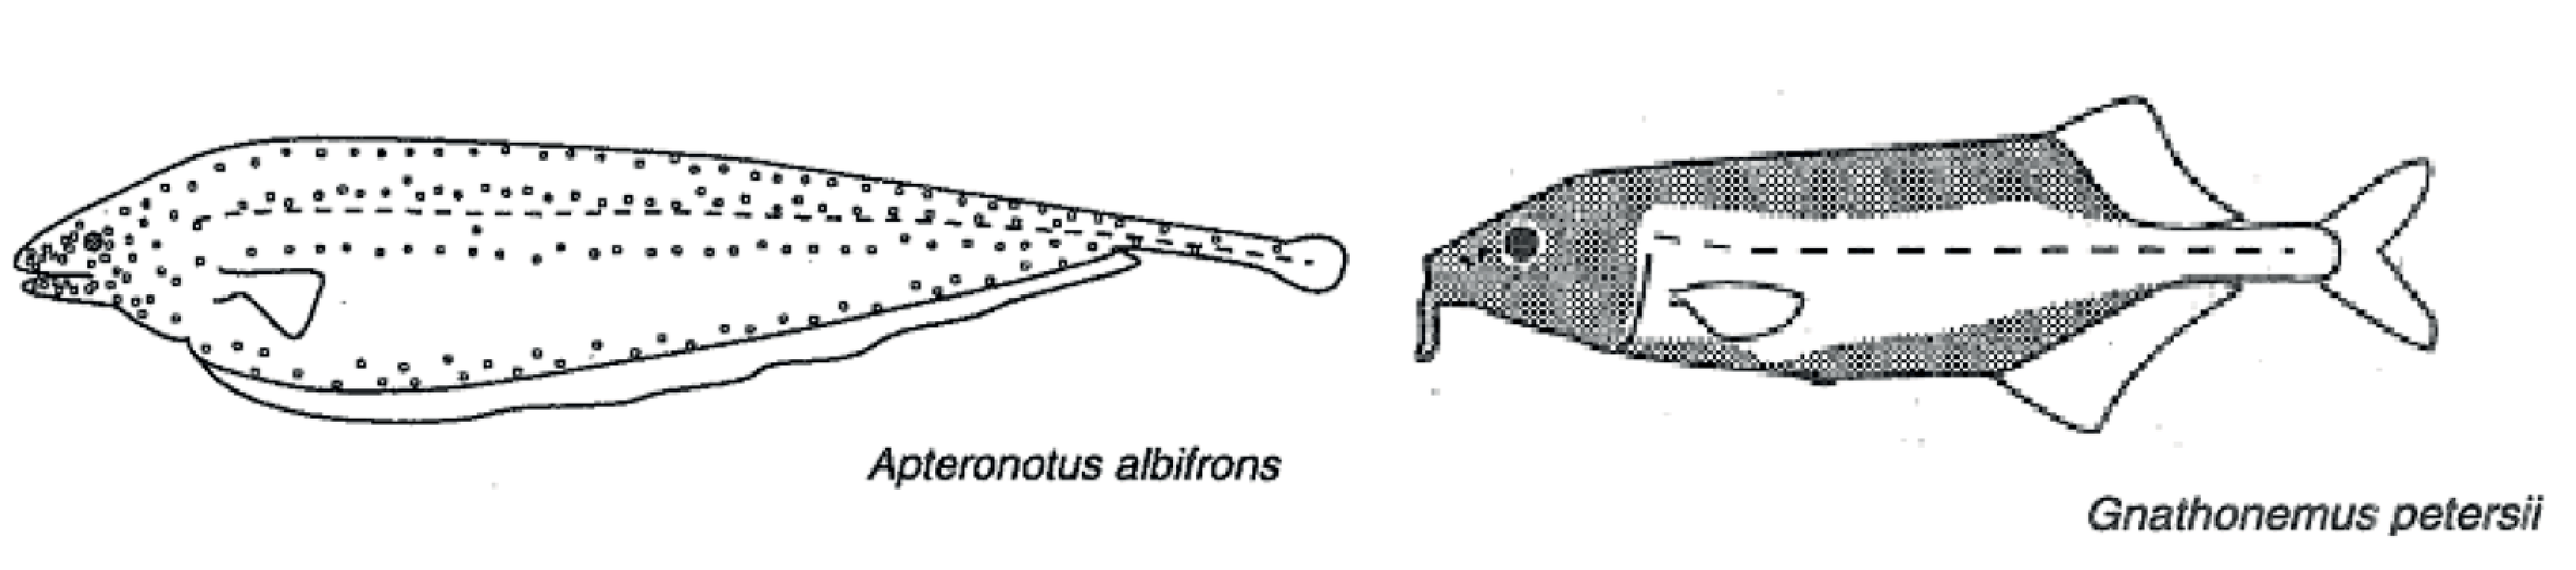
\includegraphics[width=13cm]{intro/figures/density_electroreceptors}
\caption{Location of the receptors according to the order: \emph{A. albifrons} is a Gymnotiform (each dot represents an ampullary organ - the tuberous ones show the same repartition but are simply in a higher number) and \emph{G. petersii} belongs to the Mormyrifoms order (the receptors are situated in the shaded area). Taken from \cite{moller1995electric}. \label{fig:density_electroreceptor}}
\end{figure}




\subsection{Electrolocation}

\label{sub:electro-localisation}

These fishes live in turbid water, mostly at night, and hunt small
preys - like insects or small fishes \cite{albert2005diversity,okedi1971food}.
The vision is useless in these conditions and they rely mainly on
their electric sense. Two behaviors are to be described in this section:
\emph{passive }electro-location and \emph{active }electro-location.


\subsubsection{Passive electro-location}

This type of detection is not exclusive to weakly electric fish: for
example sharks and rays also use it \cite{adair1998detection,kalmijn-1988}.
From the point of view of evolution, it seems to be anterior to active
electro-location \cite{lissmann1958evolution}. It is based on the
detection of the low frequencies of the electric field emitted by
external sources (physical, chemical or biological \cite{kalmijn-1988}).
Experimentally, it can be observed when the fish is in the field of
an electric dipole \cite{hopkins-passive}: it tends to align its
body with the streamlines and to follow it until the source (see Figure
\ref{fig:behavior_passive_electro-location}). Consequently, this
behavior does not involve a complex analysis of the electric field
and the fish does not seem to know by advance where is the dipole.
Since it is well understood, we will not study it.

\begin{figure}[h]
\centering
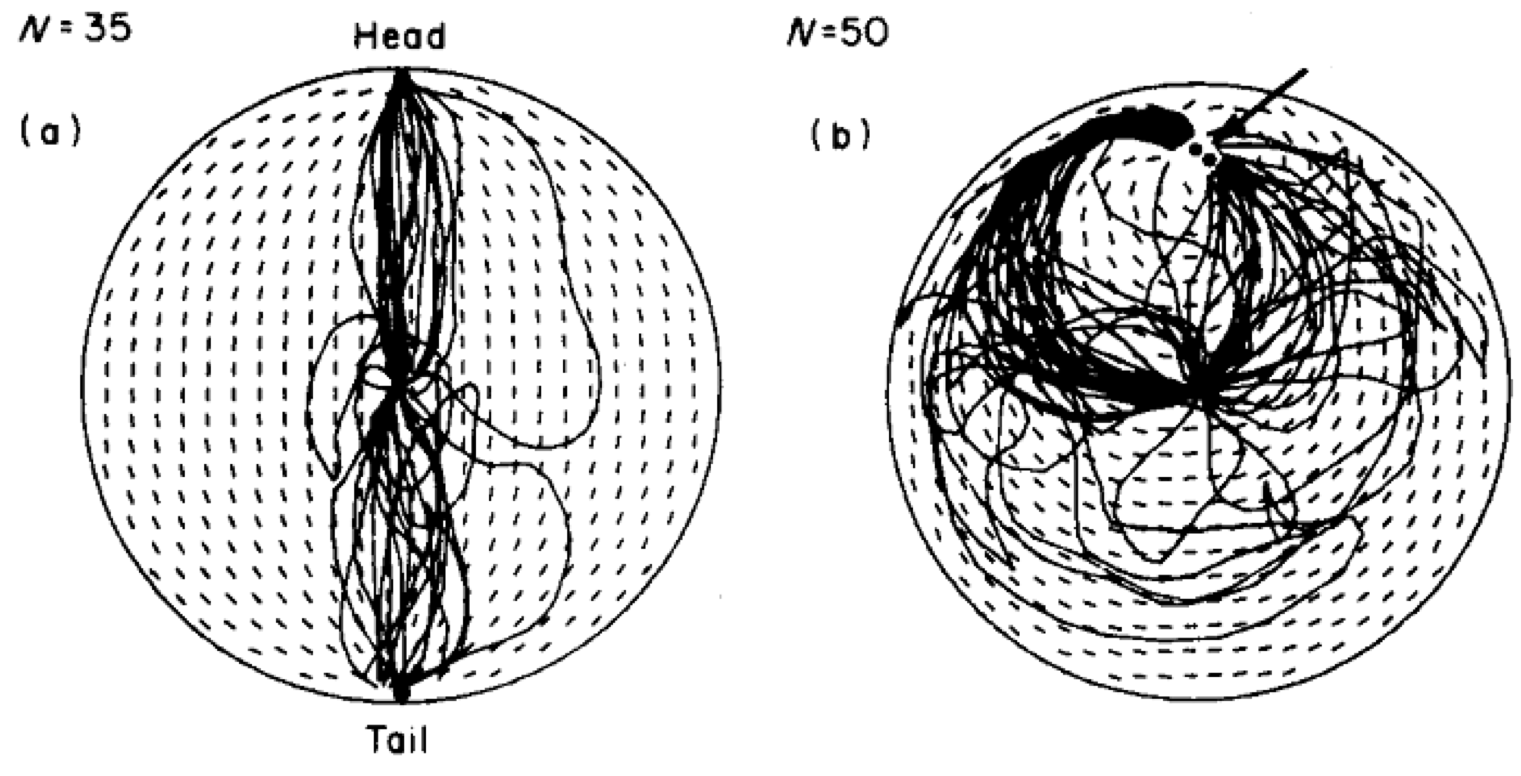
\includegraphics[width=12cm]{intro/figures/passive_electrolocation}
\caption{Behavior of \emph{G. carapo} in the presence of a dipole, with two
different geometries. Full lines correspond to pathway followed by
the fish during an essay ($N$ is the number of essays) and doted
lines are stremlines of the electric field. Taken from~\cite{davis1988behavioural}.\label{fig:behavior_passive_electro-location}}
\end{figure}



\subsubsection{Active electro-location}
\label{eq:active-electroloc-intro}

Active electro-location is far more complex because the fish seems
to know away from the object its location and its properties. It has
long been known that weakly electric fishes react strongly when a
metallic rod enters the aquarium %
\footnote{In fact it has been known since the 18$^{th}$ century, when electrogenesis was discovered
\cite{moller1995electric}.}. But it took centuries to understand why: in 1958, Hans Lissmann
finally connected this fact with their emission of a weak electric
field and concluded that they possess an ``electric sense''. This
sense has a range of about one or two body length. Behavioral studies
showed that these fishes are able to determine the distance (Figure
\ref{fig:distance_discrimination}A), the size, the shape (Figure
\ref{fig:distance_discrimination}B) and the material (via resistivity
and capacitance) of an object \cite{von1999active,von1992electro-location,von1993electric}.

\begin{figure}[h]
\centering
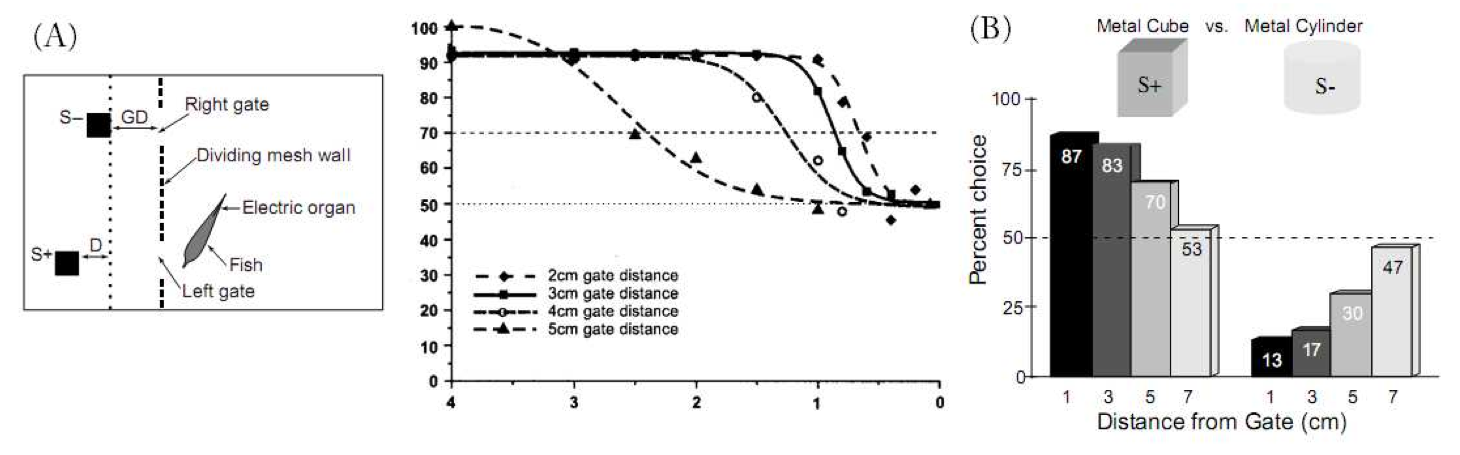
\includegraphics[width=\textwidth]{intro/figures/behavior_exp}
\caption{(A) Experimental evidence of distance measurement by a \emph{Gnathonemus
petersii}. On the left: experimental setup. The fish is forced to
enter one of two gates where objects $S^{+}$ and $S^{-}$ are placed.
These objects only differ by their distance $D$ with respect to the
gate. If the first one is chosen, the fish is rewarded (by feeding)
and if not, the fish is punished (by disturbing it). On the right
is plotted the rate of correct choice as a function of $D$. The objects
$S^{+}$ and $S^{-}$ are metallic sphere with a volume of $33.5$
cm$^{3}$. (Taken from \cite{von1993electric}). \protect \\
 (B) Experimental evidence of shape discrimination by individuals
of the same specie. The experimental setup is the same, except that
the difference between the objects is now their shape: one is a metallic
cube whereas the other is a metallic cylinder. (Taken from \cite{gerhard}).
\label{fig:distance_discrimination}}
\end{figure}

The physical principle of electro-location has been known since its
discovery by Lissmann in 1958 \cite{lissmann1958mechanism}:
the electric field's amplitude and frequency are modified when there
is an element in the surrounding with conductivity and capacitance
- respectively - different from that of the water. This modification
is then felt by tuberous receptors all over the skin and the fish
analyzes this data. However, no one knows an algorithm that can translate
this data into information on the object.

It should be noticed that when the fish probes its environment, is
exhibits an intense activity \cite{lannoo1993electric}. Moreover,
the swimming patterns are quite uncommon. For example, Gymnotiforms
do not have caudal nor dorsal fin so swimming depends entirely on
their anal fin; the result is that they can swim either forward or
backward without difficulty. The strategy used during exploration
has been called \emph{Probing Motor Acts} by Toerring and Belbenoit~\cite{toerring1979motor}:~see
Figure~\ref{fig:pma}. 
\begin{figure}[h]
 \centering
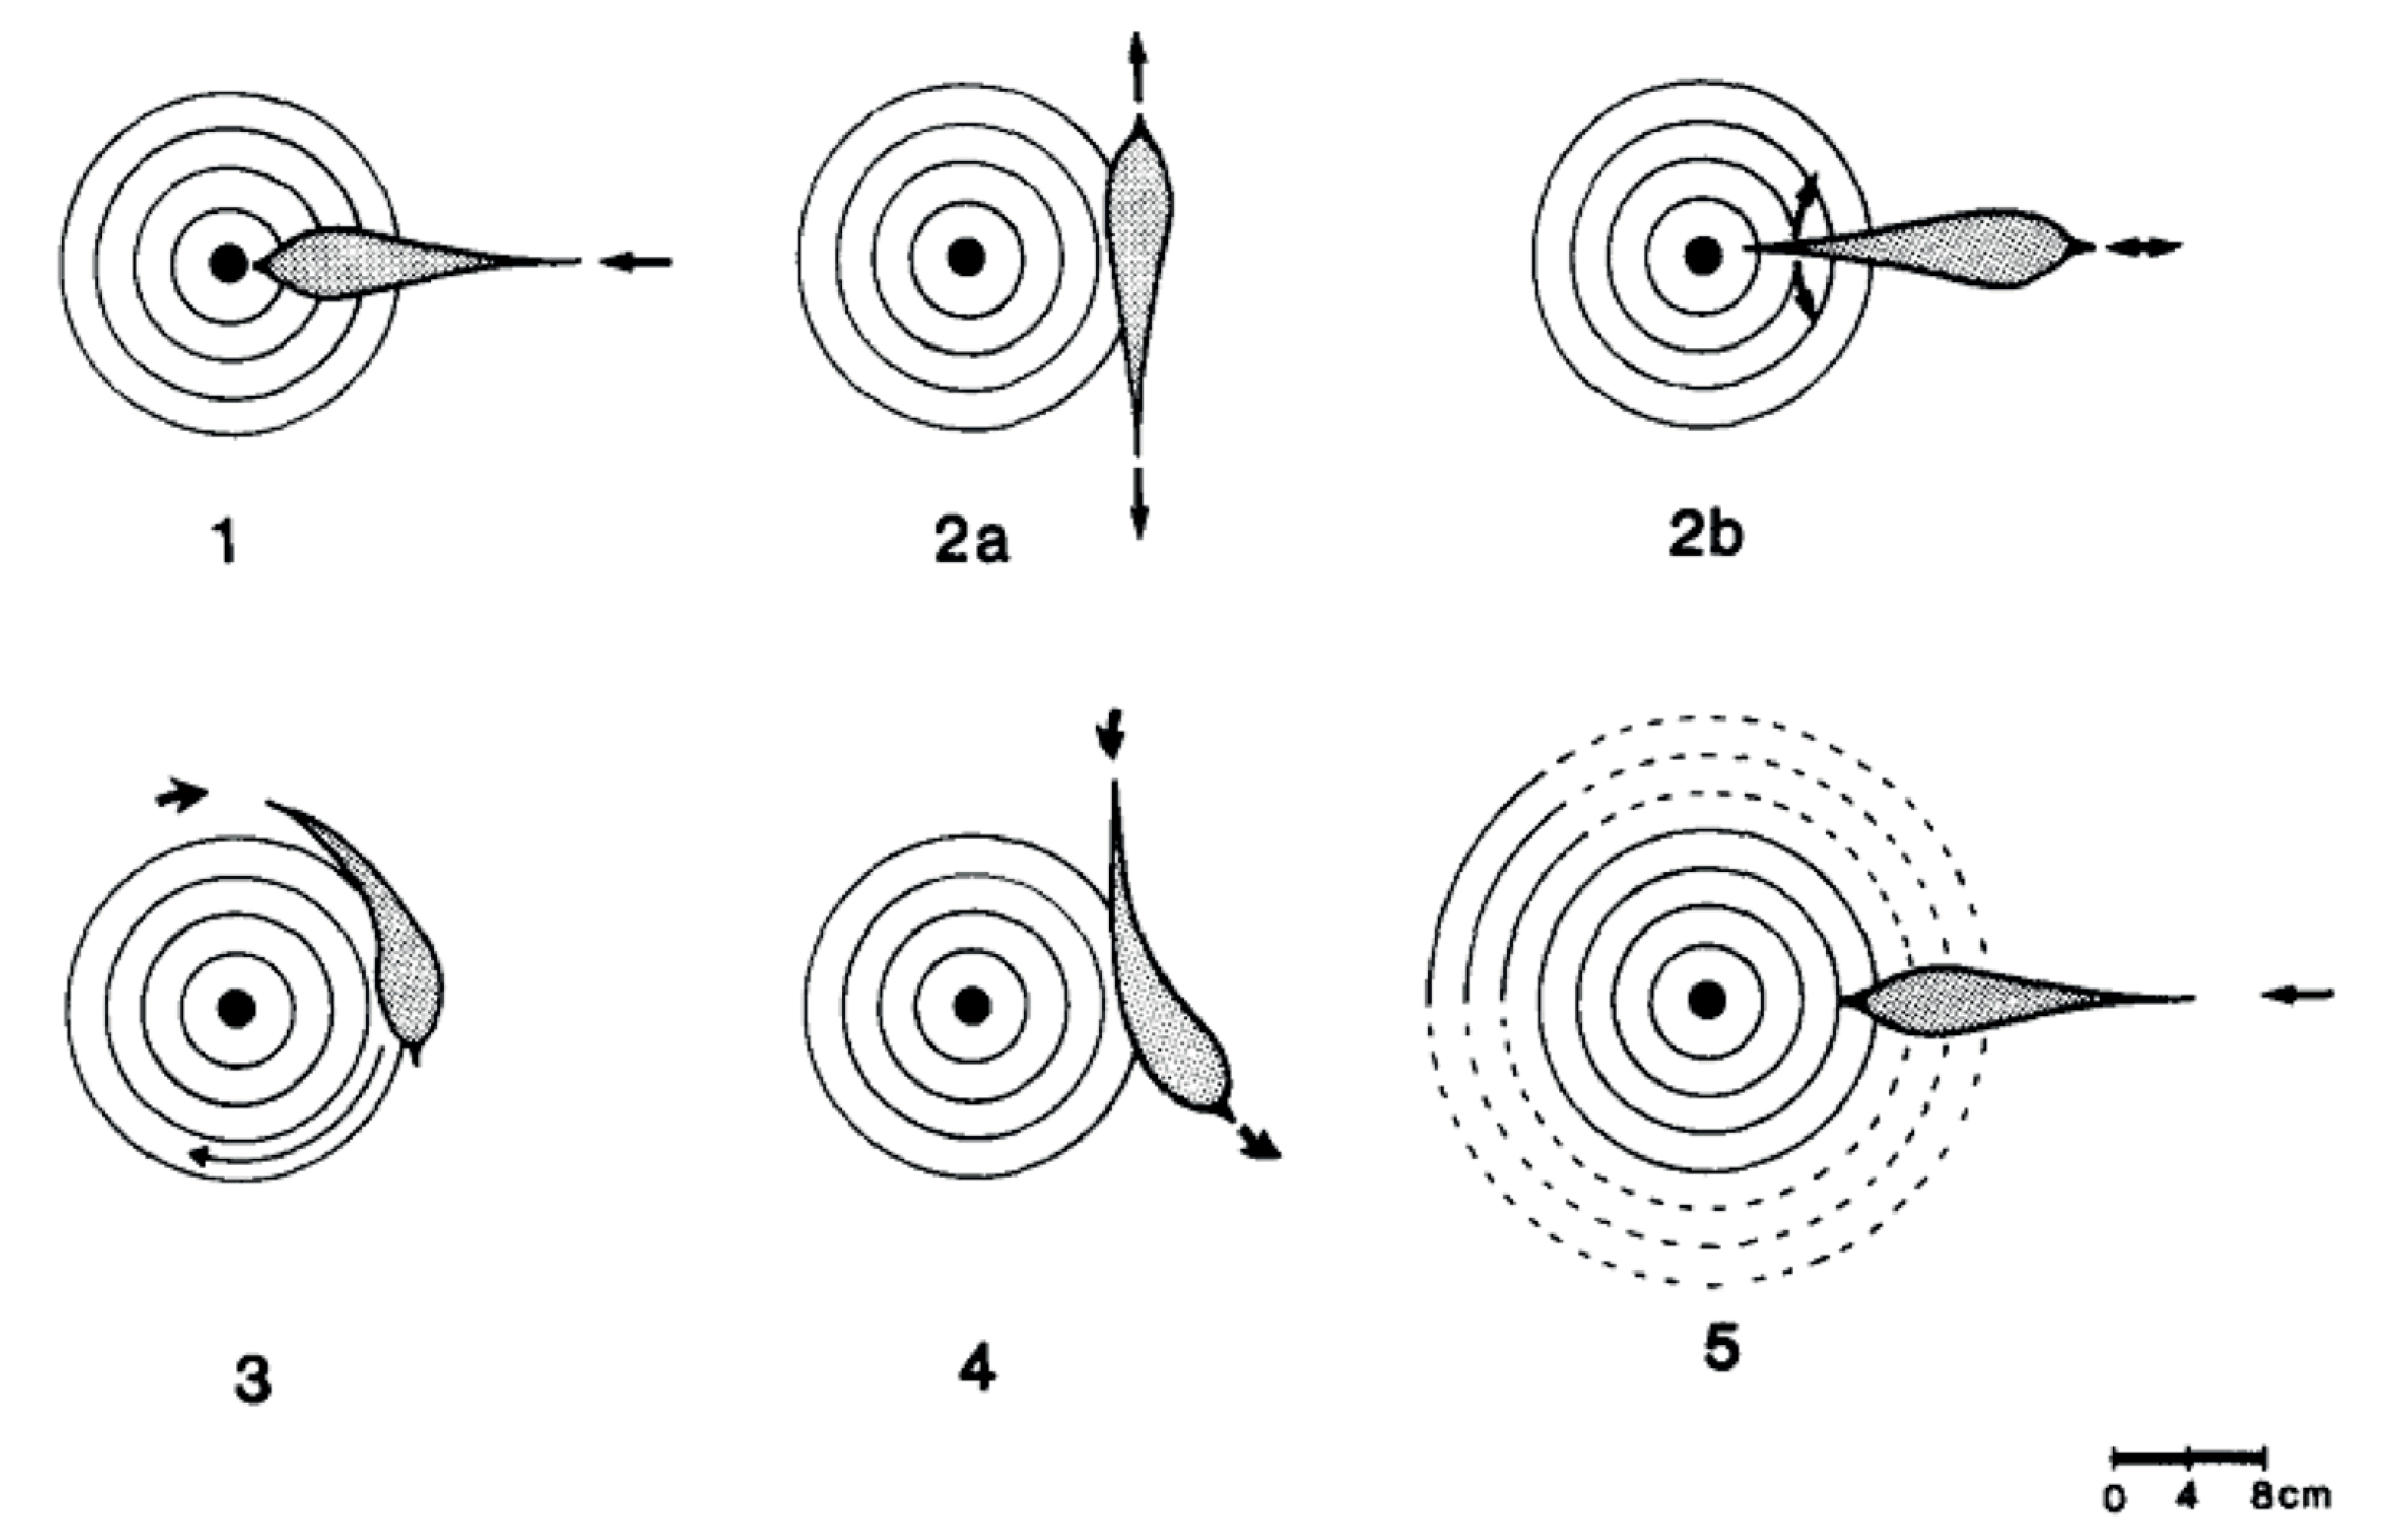
\includegraphics[width=10cm]{intro/figures/PMA}
 \caption{PMA: behavior exhibited by mormyrids (\emph{Marcusenius cyprinoides
}and \emph{Gnathonemus petersii}) when introducing a metallic - or
plastic - object (showed by the black dot). 1.~chin probing 2a.~lateral
``va-et-vient'' 2b.~radial ``va-et-vient'' 3.~lateral probing
4.~tangential probing 5.~stationary probing. Taken from \cite{toerring1984locomotor}.\label{fig:pma}}
\end{figure}


During the exploration, pulse-type species control the EOD rate by
stabilizing the frequency (see Figure \ref{fig:EOD_stabilization}).
In both types, an amplitude enhancement is also observed. A special
care will be made on these strategies when modelling the problem.

\begin{figure}[h]
\centering
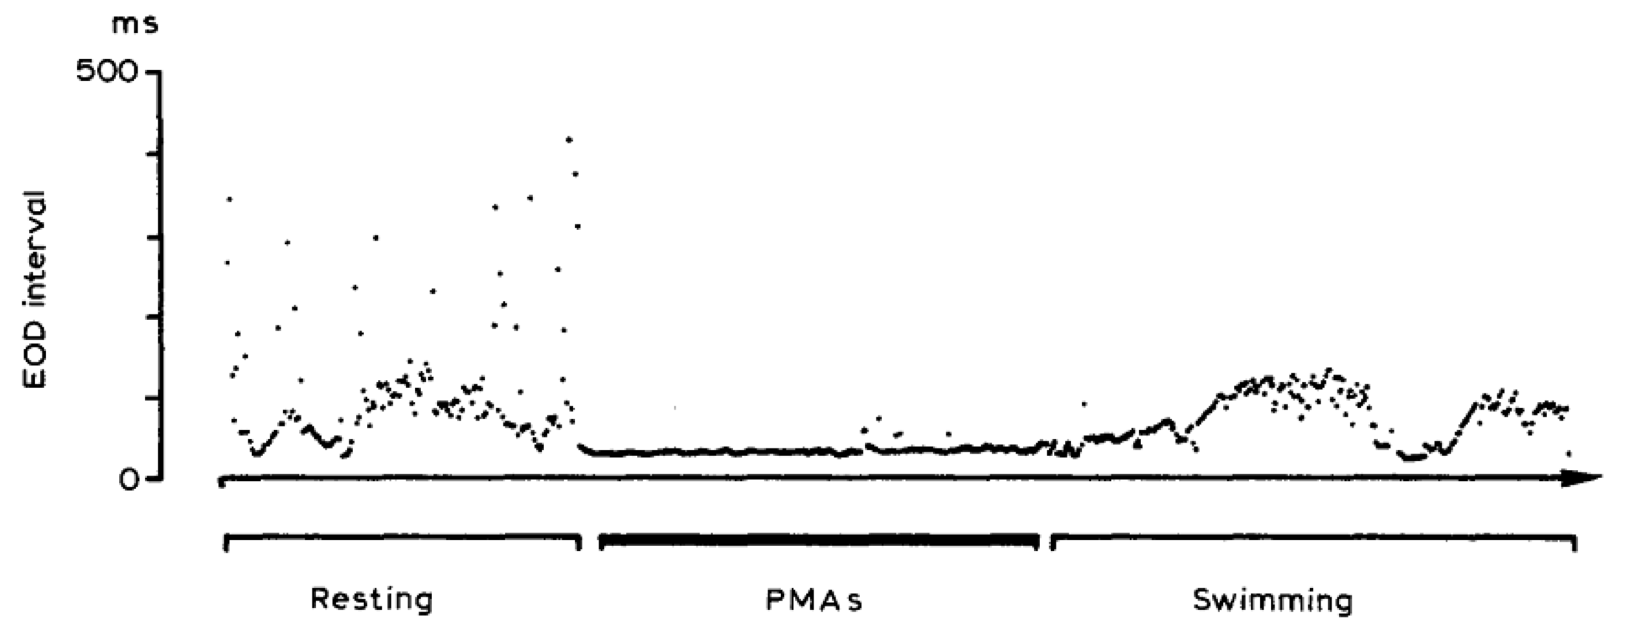
\includegraphics[width=\textwidth]{intro/figures/EOD_PMA}
\caption{EOD rate as a function of the fish's activity. Taken from \cite{toerring1984locomotor}.
\label{fig:EOD_stabilization}}
\end{figure}



\subsubsection{Modelling the electric field}

\label{sub:modelisation_champ_bio}

Electro-location has been quantitatively investigated since it is
known: in their article, Lissmann and Machin tried an analytical approach
by calculating the distortion of a dipole's electric field caused
by an infinite cylinder \cite{lissmann1958mechanism}. This section
will give a brief state-of-the-art of the progress that has been made
since then. First, we will focus on analytical results, and various
numerical approaches of the electric field will follow.

Formulas have been established to compute the effect of a scatterer
in the fish's field by several authors: Lissmann and Machin in 1958
\cite{lissmann1958mechanism}, Bacher in 1983 \cite{bacher1983} and
Rasnow in 1996 \cite{rasnow1996simple}. All of them rely on the fact
that a sphere placed in a uniform electric field ``creates'' another
field equivalent to a dipole's one. Let us see in detail what are
these formulas. In the first article, an infinite cylinder with conductivity
$\sigma$ is illuminated in a medium of conductivity $\sigma_{0}$
by a dipole $M$. In the plane, the equivalent dipole $M'$ of the
cylinder is given by the following expression (with the notation
of Figure~\ref{fig:modele_lissmann}):

\begin{equation}
\frac{M'}{M}=a^{2}\left(\frac{\sigma_{0}-\sigma}{\sigma_{0}+\sigma}\right)\frac{1}{r_{1}r_{2}}\label{eq:dipole_lissmann}
\end{equation}


\begin{figure}
\centering
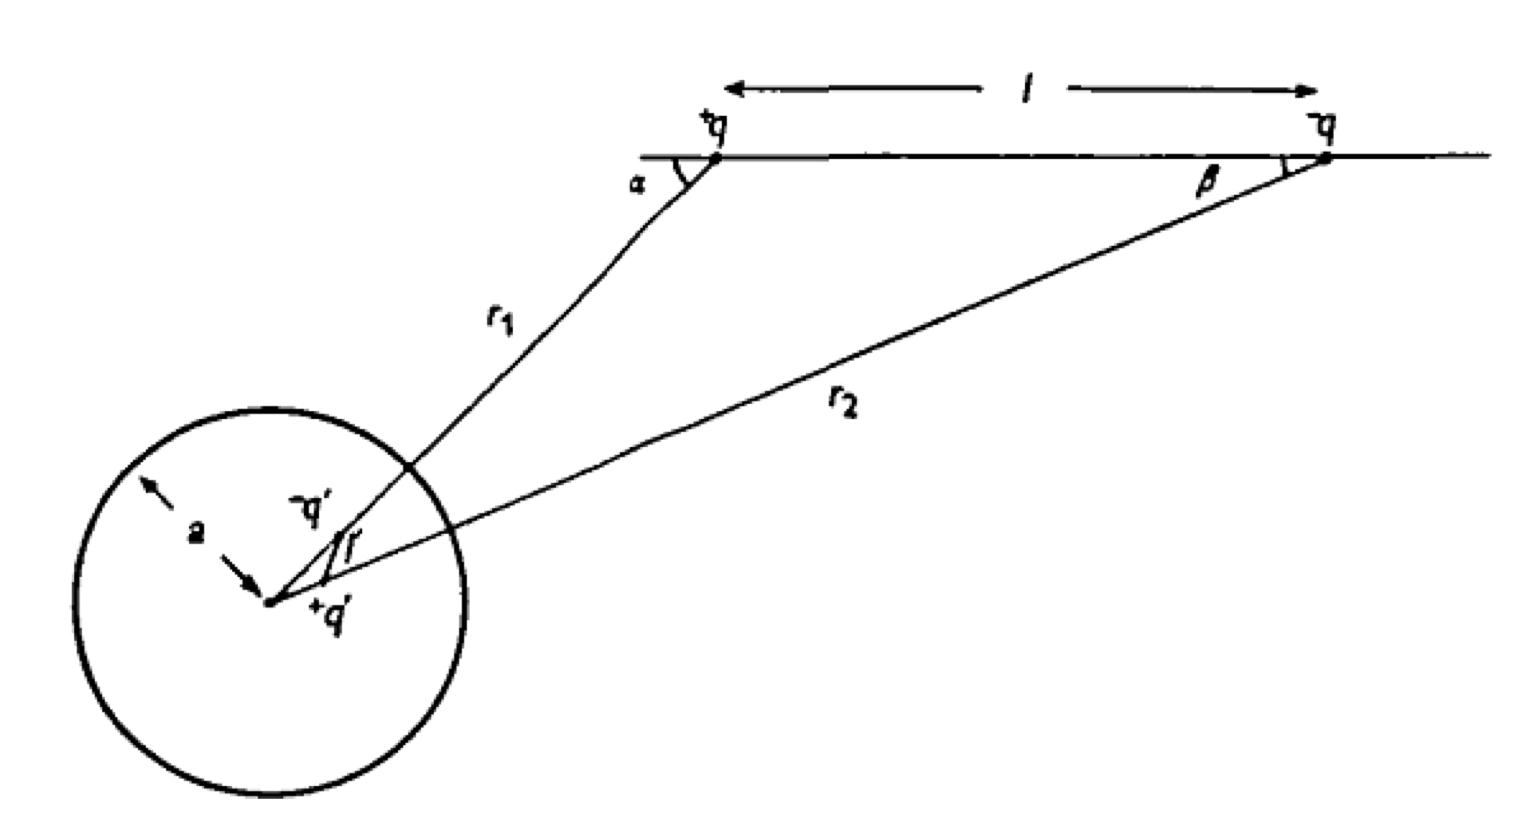
\includegraphics[width=\textwidth]{intro/figures/dipole_Lissmann}
\caption{Model used by Lissmann and Machin. An infinite cylinder of radius
$a$ is in the neighborhood of a dipole formed by two sources $+q$
and $-q$ which are separated by a distance $l$. Taken from \cite{lissmann1958mechanism}.
\label{fig:modele_lissmann}}
\end{figure}


In 1983, Bacher remarks that this formula cannot explain the phase
difference observed when the electric permittivity of the target does
not equal the water's permittivity \cite{bacher1983}. This phase
difference is important since it is measured by RT units receptors
(see section~\ref{sub:electrorecepteurs}). He proposes then to take
this into account in the equations by considering a non-stationary
electric field, but does not give a formula similar to (\ref{eq:dipole_lissmann}).
Rasnow resolves this problem in 1996 by considering a harmonic regime
for the background electric field: in the presence of a sphere of
radius $a$, conductivity $\sigma_{1}$ and permittivity $\varepsilon_{1}$,
a uniform harmonic electric field $E_{0}$ with frequency $\omega$
is modified in this way:
\begin{equation}
\delta u(\boldsymbol{r})=\boldsymbol{E_{0}}\cdot\boldsymbol{r}\left(\frac{a}{r}\right)^{3}\frac{\left(\sigma_{1}+i\omega\varepsilon_{1}\right)-\left(\sigma_{0}+i\omega\varepsilon_{0}\right)}{2\left(\sigma_{1}+i\omega\varepsilon_{1}\right)+\left(\sigma_{0}+i\omega\varepsilon_{0}\right)},
\label{eq:dipole_rasnow}
\end{equation}
 where the indices $0$ refers to the ambient medium. As we will see
in chapter~\ref{chap:math-model},
it corresponds to the first order approximation of the potential $u$
that verifies the equation $-\nabla\cdot(\sigma+i\omega\varepsilon)\nabla u=0$
where $\sigma$ (resp. $\varepsilon$) is equal to $\sigma_{1}$ (resp.
$\varepsilon_{1}$) in the sphere and $\sigma_{0}$ (resp. $\varepsilon_{0}$)
in the exterior. Let us remark that the factor in formula (\ref{eq:dipole_rasnow})
is opposed to the one in (\ref{eq:dipole_lissmann}) because the vector
$\boldsymbol{r}$ does not point at the same direction, and the factor
$2$ in the denominator is due to the fact that we are now in the
whole space and not only in the plane (see section~\ref{sub:dipolar-expansion},
Proposition~\ref{propos2}). Even if the model
has been improved, it is only correct in an ideal case: the target
is a sphere and the field is supposed to be uniform. It is not reasonable
because for example the latter assumption is not true around the tail
\cite{assad1998electric,assad1999electric}. The next section will
show how the tools developed recently in mathematical imaging can
handle it.

Numerical approaches have also been made since the 70's: in 1975,
Heiligenberg proposes a finite differences scheme to calculate the
field created by the fish \cite{heiligenberg1975theoretical}. In
1980, Hoshimiya~\emph{et al.} use finite elements to solve this problem
\cite{hoshimiya1980theapteronotus}. The geometry of the fish is simplified
by an ellipse and is divided into two areas: the thin skin with low
conductivity and the inside of the body. Their aim is to optimize
conductivity values to approximate as well as possible the experimentally
measured field. The result is that the optimal conductivity is non-uniform,
being higher in the tail region (see Figure \ref{fig:skin_resistance_hoshimiya}).

\begin{figure}
\centering
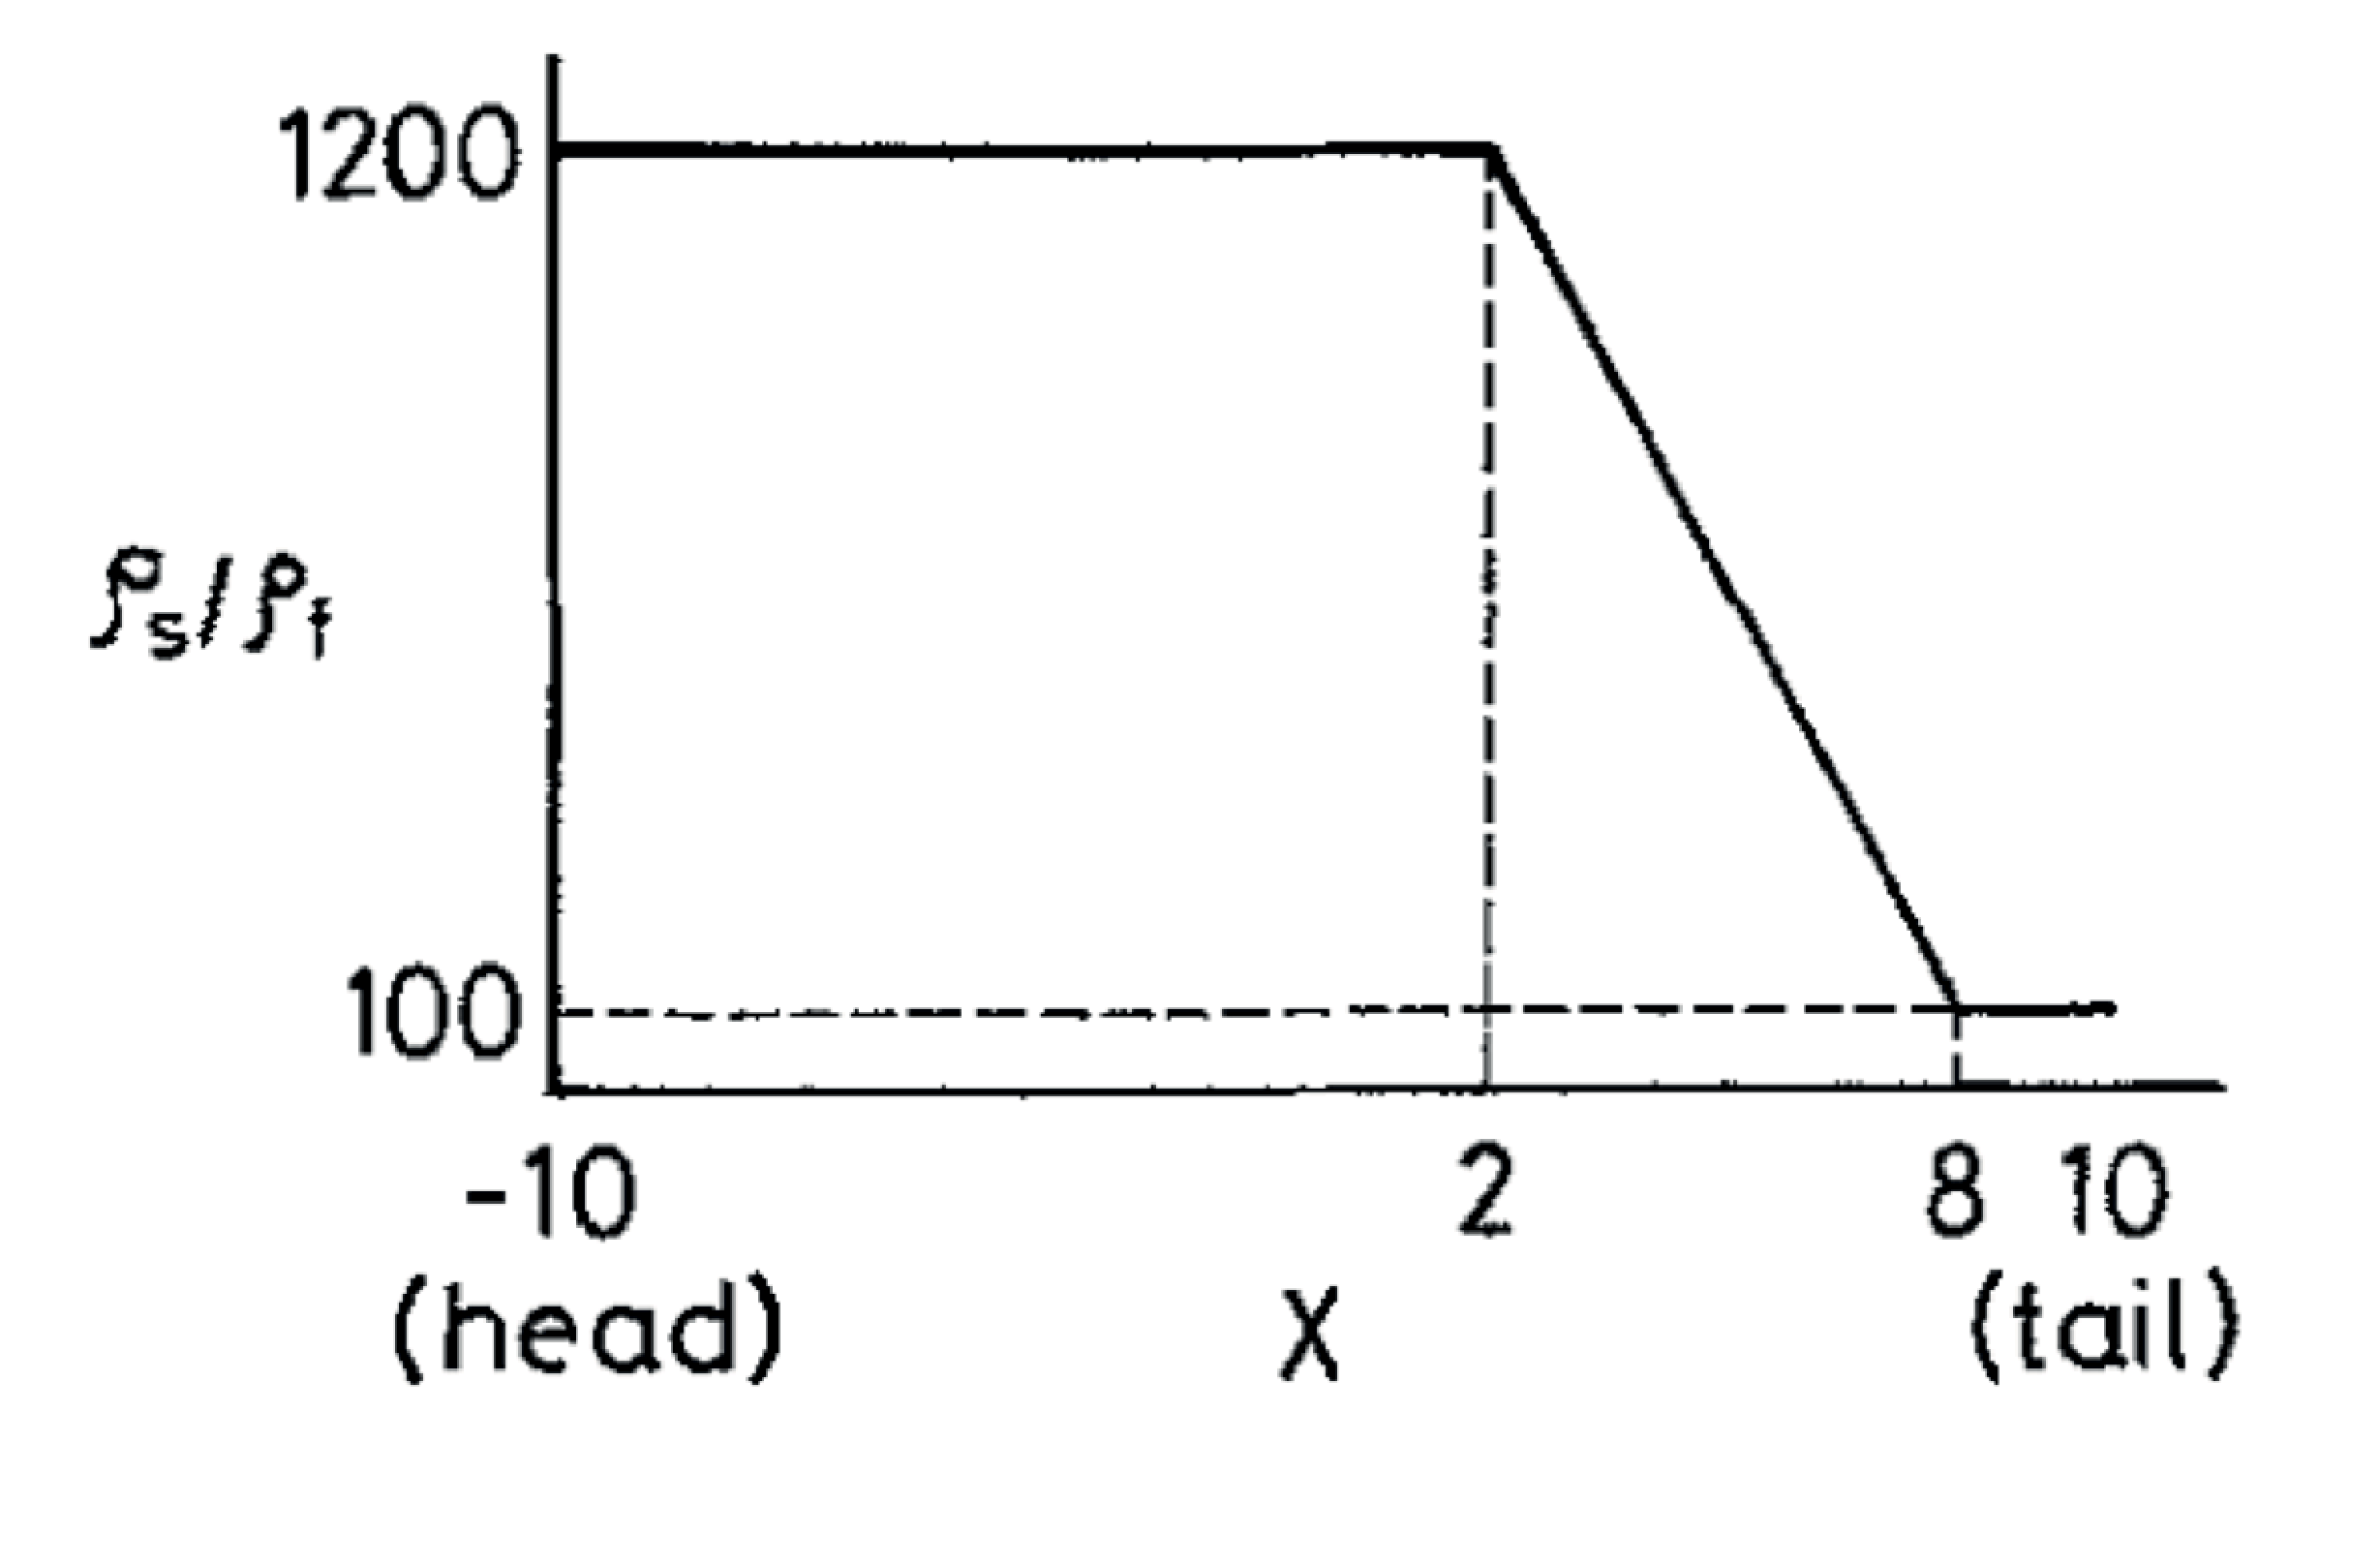
\includegraphics[width=8cm]{intro/figures/impedance_skin}
\caption{Optimal repartition of the ratio between skin resistivity $\rho_{s}$
and body conductivity $\rho_{f}$ along the head-tail axis. Taken
from~\cite{hoshimiya1980theapteronotus}. \label{fig:skin_resistance_hoshimiya}}
\end{figure}


A lot of improvement has been made since this study (see for example
\cite{babineau2006modeling,maciver2001computational,migliaro2005theoretical,rasnow1989simulation}).
It is now well-accepted that the skin conductivity is not uniform
(higher in the head) but remains low with regards to the water conductivity,
and that the body conductivity is high. According to Migliaro \emph{et al.}
\cite{migliaro2005theoretical}, the first fact increases the sensitivity
of the skin by enhancing the voltage difference and the second extends
and makes uniform the potential near the skin (which is indeed experimentally
measured \cite{nelson-target}). The relative error between measures
and simulations is around $10$\%.

Another promising technique is the use of the boundary elements method
performed by Assad in 1997 \cite{assad1997phd}. Indeed the
important feature is the electric potential on the skin (because it
is the \emph{input} for the fish), so a BEM approach allows us to
concentrate the equations on it. Moreover, the speed of calculation
is enhanced because the number of nodes is dramatically reduced. The
equation considered is here $\Delta u=0$ on the exterior of the body
with Robin boundary conditions on the skin~\cite{williams1990hypercube}:
\begin{equation}
u-\xi\frac{\partial u}{\partial n}=\psi,\label{eq:CL_assad}
\end{equation}
 where $\psi$ is the potential inside the body and $\xi=h\left(\sigma_{0}/\sigma_{s}\right)$
($h$ being the skin thickness, $\sigma_{s}$ the skin conductivity
and $\sigma_{0}$ the water conductivity) is the \emph{effective skin
thickness}. In the next section we will show the validity of this
model, which allows us to easily simulate the PMA(see Figure~\ref{fig:simulation_bem_assad}).

\begin{figure}
\centering
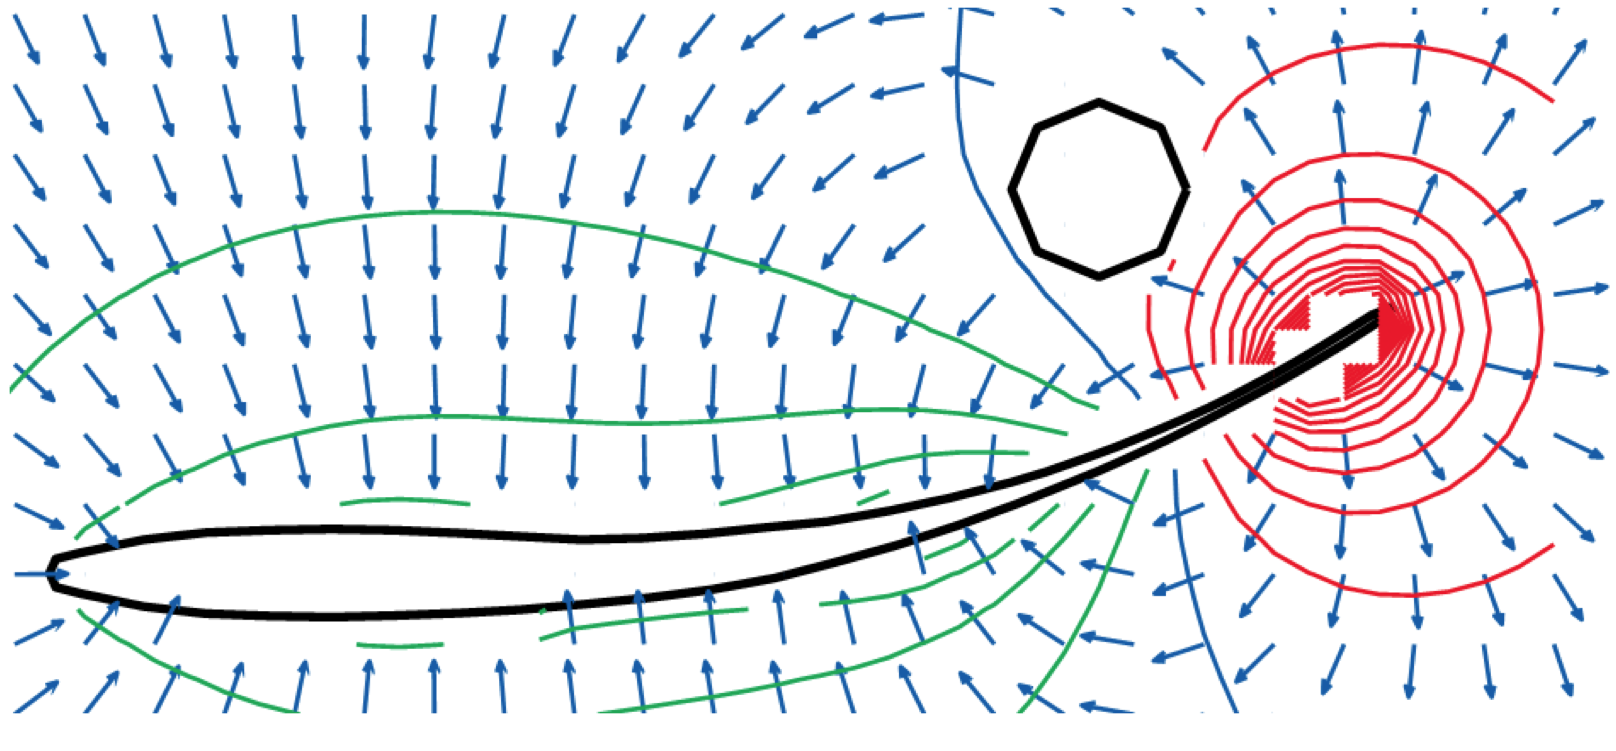
\includegraphics[width=\textwidth]{intro/figures/BEM_Assad}
\caption{BEM simulation of the field with an object, the fish's body being
curved. Isopotentials are depicted by lines ($1$ mV between each
one) and the normalized arrows indicate streamlines. Taken from \cite{assad1998electric}.
\label{fig:simulation_bem_assad}}
\end{figure}


Let us notice that there are other kinds of simulations, based on a
more empirical approach, determining an equivalent electric circuit
\cite{budelli2000electric,caputi1998electric} or an equivalent multipole
\cite{chen2005modeling}.

To conclude this section, we have seen that weakly electric fish are
able to collect data issued from their self-generated electric field,
and to analyze them in order to determine features of scatterers around
them. So far, numerical studies have been made to compute this electric
field but with a lot of differences in their approaches. Our goal
here is to analyze quantitatively the equations in order to have a
precise forward problem.


\section{Overview of the Thesis}

\label{sec:overview}

\subsection{Interests and Potential Applications}

Even if neuroethology of weakly electric fish is well developped~\cite{neuro},
knowing the neural mechanisms of active electrolocation is far beyond the scope
of mathematical modeling. Instead, we should restrict ourselves to a more accessible question. 
For example, knowing what could be the physical mechanisms is of major importance for several
reasons.

The first one is of course biological. Indeed, it is a sixth sense unknown by
a majority of species; its study unravel marvelous mysteries of Nature.

Bio-inspired engineering is the major motivation for such investigation. As a matter
of fact, autonomous water navigation is the closest application of study~\cite{boyer}.
Indeed, it would have numerous applications, for example for naval mines or UXO
(UneXplored Ordnances) detection, oceans and lakes monitoring, etc. But it would have
also other applications, going from medical to geophysical imaging. In fact, as it will be shown
in chapter~\ref{chap:math-model}, we are in the context of Electrical Impedance Tomography.
Since it is knwon for poor resolution, the performance of our fishes (see section~\ref{eq:active-electroloc-intro})
are quite impressive. Imitating their strategies would surely made improvements
for this field. 

And, last but not least, mathematical sciences would benefit for such
knowledge, since it is an inverse problem.
Indeed, given the current distribution
over the skin, the problem is to recover the conductivity distribution
in the surrounding space. Due to the ill-posedness character of this
type of problems, it is intriguing to see how much information is
the fish able to recover. Thus, modelling this ``electric
sense" (called active electrolocation) is likely to give us insights
in this regard.

Hence, this will be the central question of the thesis: how can we explain
physically the process of active electrolocation~? How it is possible to
locate and differentiate different objects situated near the fish~? 

\subsection{Organization of the Thesis}

We propose to answer these questions by means of numerical analysis of the
equations involved in the description of the self-generated electric field.

In chapter~\ref{chap:math-model}, we derive these equations and reduce them
to a simplified model, taking advantage of the highly resistive skin and
highly conductive body. A dipolar expansion of the transdermal potential
is also computed when a small target is present.

In chapter~\ref{chap:localization}, an algorithm of localization is designed.
It uses the fact that the fish emits several frequencies; thus, we can locate
a target even if the fish is static.

In chapters~\ref{chap:GPT-extraction}-\ref{chap:tracking}, we develop new
tools for extracting the relevant geometrical and physical features of the target.
Since it was not performed before, they are described in a more general framework.
In chapter~\ref{chap:GPT-extraction} the problem of extraction is derived and 
analyzed. In chapter~\ref{chap:dico-matching}, it is used for shape identification
from a pre-computed dictionary. Finally, in chapter~\ref{chap:tracking}, it is
used for tracking a mobile target.

In chapter~\ref{chap:pnas}, we gather all these tools in order to explain how
discriminating objects of different shapes could be possible. The key points
are the multi-frequency aspect of the electric field, and the movement of the fish,
thus giving sense to the PMA described in subsection~\ref{eq:active-electroloc-intro}.

The chronological order of research has been kept on purpose, taking the risk of
having to repeat the notation of chapters~\ref{chap:math-model}-\ref{chap:localization}
when returning to the physical model in chapter~\ref{chap:pnas}. Indeed, since
the first two chapters represent modeling and localization, whereas
chapters~\ref{chap:GPT-extraction}-\ref{chap:pnas} deal with shape recognition,
this order appears to be more natural.









